\documentclass[12pt, a4paper]{article}
\usepackage{amsfonts, amssymb,amsmath}
\usepackage{graphicx}
\usepackage{dsfont}
\usepackage[margin=1.0in]{geometry}
\linespread{1} 

\title{PHYC 3590 - Advanced Classical Mechanics\\Assignment 1}
\author{Gavin Kerr\\B00801584}
\date{2022-01-16}


\begin{document}

\maketitle

\section*{Question 1.16}
\subsection*{(a)}
Show that $|r| = \sqrt{r\cdot r}$. 
\begin{align*}
r =& x\hat{x} + y \hat{y} + z \hat{z}
\\
r\cdot r =& (x\hat{x} + y \hat{y} + z \hat{z})(x\hat{x} + y \hat{y} + z \hat{z})
\\
r\cdot r =& x^2 + y^2 + z^2 
\\
r\cdot r =& r^2
\\
\sqrt{r\cdot r} =& \sqrt{r^2}
\\
\sqrt{r\cdot r} =& |r|
\\
&\text{QED}
\end{align*}
\subsection*{(b)}
Prove that $r\cdot s$, as defined by (1.7), is the same for any choice of orthogonal axes. 
\begin{align*}
|r+s|^2 =& (r+s)(r+s) 
\\
(r+s)(r+s) =& r^2 + 2r\cdot s + s^2
\\
|r+s|^2 =& r^2 + 2r\cdot s + s^2
\\
2r\cdot s =& |r+s|^2 - r^2 - s^2
\\
r\cdot s =& \tfrac{1}{2}(|r+s|^2 - r^2 - s^2)
\end{align*}
All of the terms are squared therefore there are all independent of the angle. 





\section*{Problem 1.26}
\subsection*{(a)}
Assuming the puck is kicked so that the position of the puck is the same as the observer at $t=0$, we have $x=0, y=v_0t$, where $v_0$ is the initial speed at which the man kicks the puck.
\subsection*{(b)}
For $S'$ relative to $S$ we have $x=v_1t, y=0$, where $v_1$ is the speed of the second observer relative to the first observer ($S$). In the $S'$ frame, the path of the puck would be $x'= -v_1t, \, y'=v_0t$. 
\subsection*{(c)}
For $S''$ relative to $S$, we have $x=\tfrac{1}{2}at^2, \, y=0$, where $a$ is the acceleration of the third observer. In the $S''$ frame, the puck follows the path $x''=-\tfrac{1}{2}at^2, \, y''=v_1t$.\\
\\
The $S$ and $S'$ are inertial reference frames. $S''$ is not an inertial reference frame because it is accelerating.





\section*{Problem 1.31}
If there is no acceleration and no change in masses then the momentum of the system, $p_1 + p_2$ is constant. This gives
\begin{align}
p_1 + p_2 =& c
\\
\frac{dp_1}{dt} + \frac{dp_2}{dt} =& \frac{dc}{dt} = 0 \label{equation1}
\end{align}
From equation (1.21) in Taylor we have:
\begin{align}
\dot{p_1} =& F_1 = F_{12} \label{f12}
\\
\dot{p_2} =& F_2 = F_{21} \label{f21}
\end{align}
Subbing equations (\ref{f12}) and (\ref{f21}) into equation (\ref{equation1}) gives
\begin{align*}
F_1 + F_2 =& 0
\\
F_1 =& - F_2
\\
\text{QED}
\end{align*}





\pagebreak
\section*{Problem 1.39}
\begin{figure}[h]
  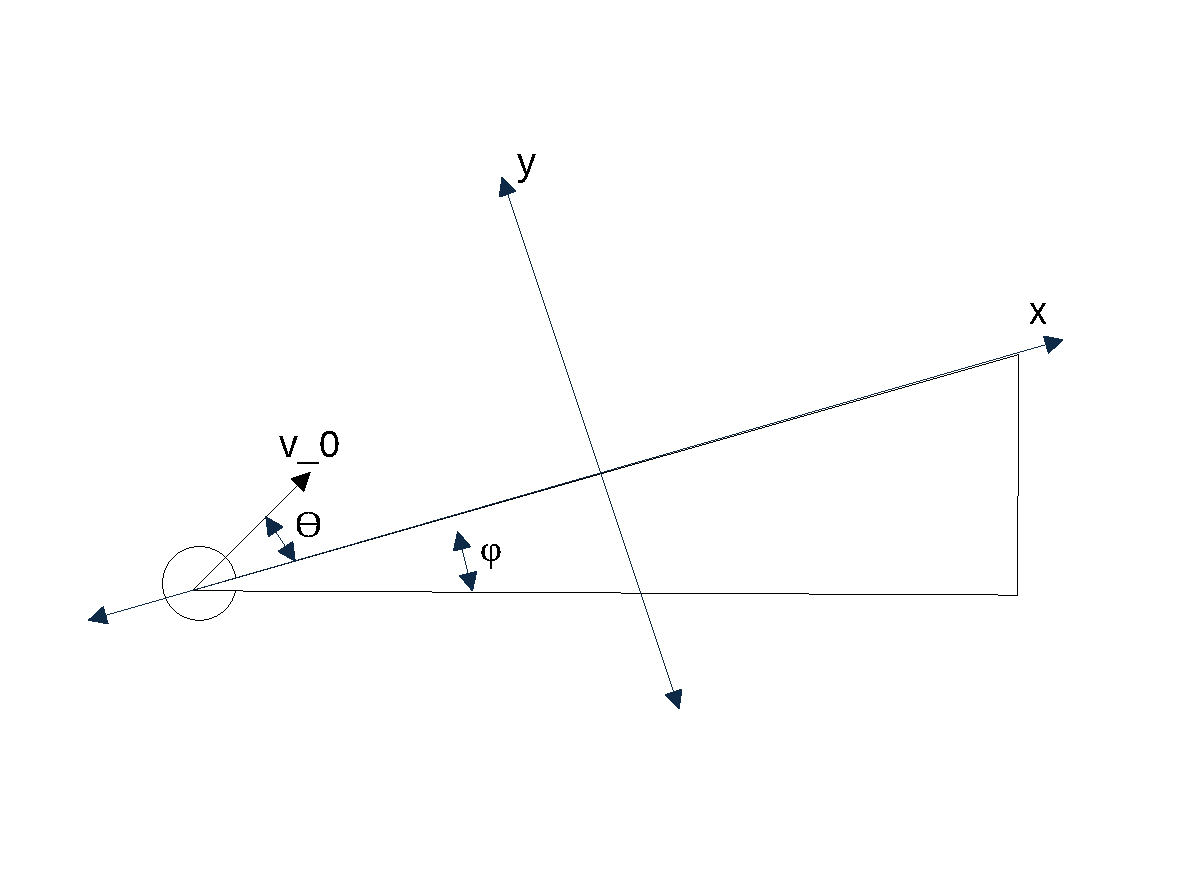
\includegraphics[width=4in]{fig_1.pdf}
  \caption{Diagram}
  \label{fig_1}
\end{figure}
For the initial conditions, we have $\vec{v_0}$. Also there is only one force acting on the object $\vec{F_g}$ which means that $\vec{g}$ is the acceleration. Solving for the equations of motion, we have
\begin{align*}
\vec{g} =& -g(\sin\phi \hat{x}+\cos\phi \hat{y})
\\
\vec{v} =& \int \vec{g} \,dt + \vec{v_0}
\\
\vec{v_0} =& v_0(\cos\theta\hat{x}+\sin\theta\hat{y})
\\
\vec{v} =& -g(\sin\phi \hat{x}+\cos\phi \hat{y})t + |v_0|(\cos\theta\hat{x}+\sin\theta\hat{y})
\\
\vec{r} =& \int \vec{v} \,dt
\\
\vec{r} =& \int -g(\sin\phi \hat{x}+\cos\phi \hat{y})t + |v_0|(\cos\theta\hat{x}+\sin\theta\hat{y}) \, dt
\\
\vec{r} =& -g(\sin\phi \hat{x}+\cos\phi \hat{y})\frac{t^2}{2} + |v_0|(\cos\theta\hat{x}+\sin\theta\hat{y})t
\\
x =& v_0\cos\theta \,t - \tfrac{1}{2}g\sin\phi \,t^2
\\
y =& v_0\sin\theta \,t - \tfrac{1}{2}g\cos\phi \,t^2
\end{align*}
Next we want to find out for how long, the ball is in the air. To do this, we need to find the difference of the two roots of the equation for $y$. The first root is trivially $t_1=0$. For the second root, $t_2 = \Delta t$, we have
\begin{align*}
0 =& |v_0|\sin\theta \,t - \tfrac{1}{2}|g|\cos\phi \,t^2
\\
0 =& |v_0|\sin\theta  - \tfrac{1}{2}|g|\cos\phi \,t
\\
\tfrac{1}{2}g\cos\phi \,t =& |v_0|\sin\theta
\\
t_2 =& \dfrac{2|v_0|\sin\theta}{g\cos\phi}
\end{align*}
This means the the ball touches the ramp at $t = \dfrac{2|v_0|\sin\theta}{g\cos\phi}$. Subbing this into the equation for $x$ to find the final position gives us
\begin{align*}
x =& |v_0|\cos\theta \left(\dfrac{2v_0\sin\theta}{g\cos\phi}\right) - \tfrac{1}{2}g\sin\phi \left(\dfrac{2v_0\sin\theta}{g\cos\phi}\right)^2
\\
x =&  \left(\dfrac{2v_0^2\sin\theta\cos\theta}{g\cos\phi}\right) -  \left(\dfrac{2v_0^2\sin^2\theta\sin\phi}{g\cos^2\phi}\right)
\\
x =&  \frac{2v_0^2}{g}\left(\dfrac{\sin\theta\cos\theta}{\cos\phi} -  \dfrac{\sin^2\theta\sin\phi}{\cos^2\phi}\right)
\\
x =&  \frac{2v_0^2}{g}\left(
\dfrac{\sin\theta\cos\theta\cos\phi}{\cos^2\phi} -  
\dfrac{\sin^2\theta\sin\phi}{\cos^2\phi}
\right)
\\
x =&  \frac{2v_0^2}{g}\left(
\dfrac{\sin\theta\cos\theta\cos\phi - \sin^2\theta\sin\phi}{\cos^2\phi}
\right)
\\
x =&  \frac{2v_0^2}{g}\left(
\dfrac{\sin\theta(\cos\theta\cos\phi - \sin\theta\sin\phi)}{\cos^2\phi}
\right)
\\
x =&  \frac{2v_0^2}{g}\left(
\dfrac{\sin\theta\cos(\theta+\phi)}{\cos^2\phi}
\right)
\\
x =& \boxed{R = \dfrac{2v_0^2\sin\theta\cos(\theta+\phi)}{g\cos^2\phi}}
\\
&\text{QED}
\end{align*}
To solve for $R_{max}$ we need to find a local max for $R$ as a function of $\theta$, where $\tfrac{dR}{d\theta}=0$.
\begin{align*}
\frac{dR}{d\theta} =& \frac{d}{d\theta}\dfrac{2v_0^2\sin\theta\cos(\theta+\phi)}{g\cos^2\phi}
\\
\frac{dR}{d\theta} =& \dfrac{2v_0^2}{g\cos^2\phi}\frac{d}{d\theta}\left(\sin\theta\cos(\theta+\phi)\right)
\\
\frac{dR}{d\theta} =& \dfrac{2v_0^2}{g\cos^2\phi}\left(
\cos\theta\cos(\theta+\phi) -
\sin\theta\sin(\theta+\phi)
\right)
\\
\frac{dR}{d\theta} =& \dfrac{2v_0^2}{g\cos^2\phi}\cos(2\theta+\phi)
\\
0 =& \dfrac{2v_0^2}{g\cos^2\phi}\cos(2\theta+\phi)
\\
\pi/2 =& 2\theta+\phi
\\
\pi/2 - \phi =& 2\theta
\\
\theta_{max} =& \boxed{\frac{\pi-2\phi}{4}}
\end{align*}
Next, we just sub $\theta$ into the equation for $R$ to find the maximum distance.
\begin{align*}
R_{max} =& \dfrac{2v_0^2\sin\theta\cos(\frac{\pi-2\phi}{4}+\phi)}{g\cos^2\phi}
\\
R_{max} =& \dfrac{2v_0^2\sin\theta\cos(\frac{\pi-2\phi+4\phi}{4})}{g\cos^2\phi}
\\
R_{max} =& \dfrac{2v_0^2\sin\theta\cos(\frac{\pi+2\phi}{4})}{g\cos^2\phi}
\\
R_{max} =& \dfrac{2v_0^2\sin\theta\cos(
\frac{\pi}{4} + 
\frac{\phi}{2}
)}{g\cos^2\phi}
\\
R_{max} =& \dfrac{2v_0^2\sin\theta
[\cos(\frac{\pi}{4})
\cos(\frac{\phi}{2}) -
\sin(\frac{\pi}{4})
\sin(\frac{\phi}{2})]
}{g\cos^2\phi}
\\
R_{max} =& \dfrac{2v_0^2\sin\theta
[\frac{\sqrt{2}}{2}
\cos(\frac{\phi}{2}) -
\frac{\sqrt{2}}{2}
\sin(\frac{\phi}{2})]
}{g\cos^2\phi}
\\
R_{max} =& \dfrac{\sqrt{2}v_0^2\sin(\frac{\pi-2\phi}{4})
[\cos(\frac{\phi}{2}) - \sin(\frac{\phi}{2})]
}{g\cos^2\phi}
\\
R_{max} =& \dfrac{\sqrt{2}v_0^2
\sin(\pi/4-\phi/2)
[\cos(\frac{\phi}{2}) - \sin(\frac{\phi}{2})]
}{g\cos^2\phi}
\\
R_{max} =& \dfrac{\sqrt{2}v_0^2
[\sin(\pi/4)
\cos(\phi/2) -
\cos(\pi/4)
\sin(\phi/2)]
[\cos(\frac{\phi}{2}) - \sin(\frac{\phi}{2})]
}{g\cos^2\phi}
\\
R_{max} =& \dfrac{\sqrt{2}v_0^2
[\sqrt{2}/2
\cos(\phi/2) -
\sqrt{2}/2
\sin(\phi/2)]
[\cos(\frac{\phi}{2}) - \sin(\frac{\phi}{2})]
}{g\cos^2\phi}
\\
R_{max} =& \dfrac{v_0^2
[\cos(\frac{\phi}{2}) - \sin(\frac{\phi}{2})]
[\cos(\frac{\phi}{2}) - \sin(\frac{\phi}{2})]
}{g\cos^2\phi}
\\
R_{max} =& \dfrac{v_0^2
[\cos^2(\frac{\phi}{2}) - 2\sin(\frac{\phi}{2})\cos(\frac{\phi}{2})+
\sin^2(\frac{\phi}{2})]
}{g\cos^2\phi}
\\
R_{max} =& \dfrac{v_0^2
[1 - 2\sin(\frac{\phi}{2})\cos(\frac{\phi}{2})]
}{g\cos^2\phi}
\\
R_{max} =& \dfrac{v_0^2
[1 - \sin\phi]
}{g\cos^2\phi}
\\
R_{max} =& \dfrac{v_0^2
[1 - \sin\phi]
}{g(1-\sin^2\phi)}
\\
R_{max} =& \dfrac{v_0^2
[1 - \sin\phi]
}{g(1-\sin\phi)(1+\sin\phi)}
\\
R_{max} =& \boxed{\dfrac{v_0^2}{g(1+\sin\phi)}}
\\
&\text{QED}
\end{align*}





\pagebreak
\section*{Problem 1.46}
\subsection*{(a)}
I don't think it's stated which direction the puck is going so we will say that the puck starts off on the west most edge of the table ($-R$) and travels east through the center of the circle. In the frame $S$, we have the equation of motion $\boxed{\vec{r} =  (v_0 - R)\hat{r} + 0\hat{\phi}}$, where $R$ is the radius of the table and $v_0$ in the initial velocity.  

\subsection*{(b)}
For the $S'$ position we have the puck starting at the same position as before, $-R$. The $\hat{r}$ vector will remain the same as the table spinning will not affect the distance between the center of the table and the puck. There will, however, be a change in the angular velocity. For the frame $S'$, there is a constant angular velocity we will call $\omega$. Combining these results, we have the equation for motion: $\boxed{\vec{v} = (v_0 - R)\,\hat{r} + \omega t \,\hat{\phi}}$.
\begin{figure}[h]
  \centering
  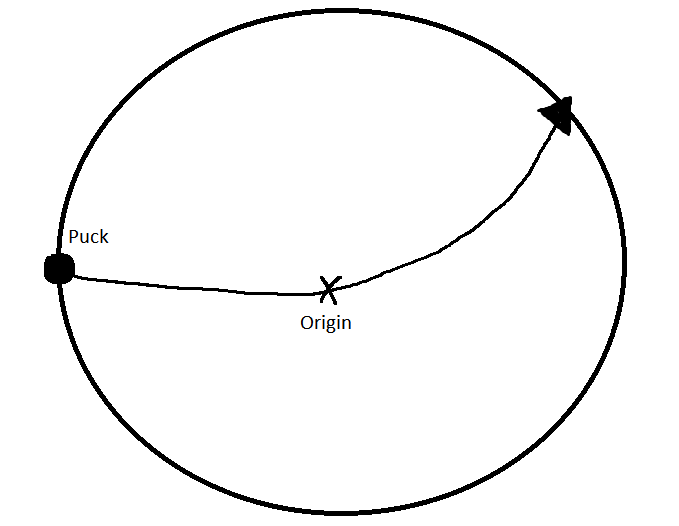
\includegraphics[width=4in]{fig_3.png}
  \caption{Shows the path of the puck from the $S'$ reference frame.}
  \label{fig_1}
\end{figure}























\end{document}
